%% Relatorio do TP "Analisando Grafos do SNAP" - formato WebMedia (ACM sigconf)
%% Compilar no Overleaf (template WebMedia) ou com: pdflatex + bibtex + pdflatex x2.
%% As figuras sao lidas de figures/ (mesma pasta) ou de ../figures/ (repositorio).
\documentclass[sigconf]{acmart}

\usepackage[brazil]{babel}
\usepackage{graphicx}
\usepackage{booktabs}
\usepackage{multirow}
\graphicspath{{figures/}{../figures/}}

%% Remove informacoes de copyright/ACM Reference do template
\settopmatter{printacmref=false}
\renewcommand\footnotetextcopyrightpermission[1]{}
\setcopyright{none}
\acmConference[WebMedia]{Trabalho Prático -- Grafos}{2026}{Salvador, BA}
\acmYear{2026}
\acmDOI{}
\acmISBN{}

\begin{document}

\title{Atenção visual em grupos de discussão: análise estrutural do grafo G16 (comm-f2f-Resistance) do SNAP}

\author{NOME COMPLETO DO(A) ESTUDANTE}
\affiliation{%
  \institution{Instituto de Computação -- Universidade Federal da Bahia}
  \city{Salvador}
  \state{BA}
  \country{Brasil}}
\email{matrícula 224215945}

\begin{abstract}
Este trabalho analisa o grafo G16 do SNAP, \textit{comm-f2f-Resistance}, que registra para onde
cada participante olha durante 62 partidas do jogo \textit{The Resistance}. O grafo original é
temporal, dirigido e ponderado, com 451 vértices e 3.126.993 arestas temporais. Ele foi convertido
em um grafo estático não dirigido de 451 vértices e 548 arestas, por meio de um limiar de atenção
relativo ao tamanho de cada partida. Calculamos as medidas estruturais obrigatórias e implementamos
e validamos BFS, DFS, verificação de Eulerianidade, Dijkstra, Bellman-Ford, Floyd-Warshall, Tarjan,
Kruskal e Prim, com análise de complexidade teórica e de tempo observado. A rede é formada por 85
componentes pequenas e densas. Não segue lei de potência. Mostra apenas indícios fracos de
small-world. Resiste à remoção aleatória de 5\% dos vértices, mas é sensível à remoção dos 5\% mais
centrais. O achado principal é a existência de um \textit{jogador focal}: em 32 das 62 partidas, há
alguém olhado acima do uniforme por todos os demais. Em 42 partidas, o mais olhado é o mesmo nos
três terços do jogo, contra 1,2 esperado ao acaso.
\end{abstract}

\keywords{teoria dos grafos, redes sociais, SNAP, small-world, lei de potência, robustez}

\maketitle

%% ===================================================================
\section{Introdução}

Este trabalho aplica conceitos da disciplina a um grafo real do repositório SNAP~\cite{snap}. Ele
cobre o tratamento dos dados, a análise estrutural (Parte~I), a implementação de algoritmos clássicos
com medição de desempenho (Parte~II) e a investigação de propriedades de redes complexas (Parte~III):
small-world, lei de potência, robustez e aproximação a modelos clássicos.

Código, dados tratados e instruções de execução estão em
\url{https://github.com/NadsonSantana/GrafoG16}. Todo o código é em Python 3.11, com
NetworkX~3.6~\cite{hagberg2008networkx}, NumPy, SciPy e Matplotlib. Os algoritmos da Parte~II e o
cálculo de small-world foram implementados sem funções prontas. O NetworkX foi usado apenas para
validar os resultados e calcular a betweenness na análise de robustez.

%% ===================================================================
\section{Determinação do grafo}

Pela regra do enunciado, o índice do grafo é
$(\textit{soma dos dígitos} \times (\textit{dois últimos dígitos} + 1)) \bmod 129$, com 0
substituído por 129. Para a matrícula $M = 224215945$:
\begin{itemize}
  \item soma dos dígitos: $2+2+4+2+1+5+9+4+5 = 34$;
  \item dois últimos dígitos: $45$;
  \item $(34 \times 46) \bmod 129 = 1564 \bmod 129 = 16$.
\end{itemize}
O grafo atribuído é o \textbf{G16}: \textit{comm-f2f-Resistance} (categoria \textit{Social networks}).

%% ===================================================================
\section{Descrição do grafo original}

O conjunto \textit{Dynamic Face-to-Face Interaction Networks}~\cite{kumar2021deception,bai2019predicting}
contém 62 redes, uma por partida de \textit{The Resistance}. Cada partida tem de 5 a 8 jogadores e
dura de 45 a 60 minutos. A cada $1/3$ de segundo, uma aresta dirigida $u \rightarrow v$ indica que
$u$ olha para $v$ ou para o laptop do jogo. Essa informação foi extraída de vídeo pelo algoritmo ICAF.
Há duas versões do conjunto: uma binária e outra ponderada pela probabilidade estimada do olhar.

A inspeção dos arquivos reproduziu exatamente as estatísticas publicadas:
\begin{itemize}
  \item 62 redes e 451 vértices (soma dos participantes);
  \item 3.126.993 arestas temporais: 2.929.953 entre jogadores e 197.040 para o laptop;
  \item 426.015 quadros, ou 142.005 segundos.
\end{itemize}
Não há valores faltantes nem auto-loops. Os jogadores nunca participam de mais de uma partida, de
modo que \textbf{as 62 redes são disjuntas}.

%% ===================================================================
\section{Tratamento realizado}

\begin{enumerate}
  \item \textbf{Temporal $\rightarrow$ estático.} Para cada partida e cada par dirigido, definimos a
  atenção $a_{uv}$ como a fração dos quadros em que $u$ olha para $v$, usando a versão binária.
  A probabilidade média da versão ponderada foi guardada como atributo; as duas medidas têm
  correlação de 0,95.
  \item \textbf{Remoções.} Descartamos as arestas para o laptop, que não é um participante. Auto-loops
  não ocorrem nos dados.
  \item \textbf{Limiar relativo.} Sem filtro, 2.867 dos 2.870 pares dirigidos possíveis aparecem, e
  cada partida vira um grafo quase completo. Por isso, mantivemos $u \rightarrow v$ apenas se
  $a_{uv} \ge 1/(n-1)$, isto é, se $u$ olha para $v$ mais do que olharia distribuindo a atenção
  igualmente entre os $n-1$ colegas. O limiar se ajusta ao tamanho de cada partida.
  \item \textbf{Dirigido $\rightarrow$ não dirigido.} Definimos a atenção mútua
  $m_{uv} = (a_{uv}+a_{vu})/2$ e aplicamos o mesmo limiar. O peso $d_{uv} = 1 - m_{uv}$ (atenção alta
  significa vértices próximos) é usado em caminhos mínimos e na árvore geradora. A versão dirigida,
  com 1.045 arcos, foi mantida para o Tarjan de componentes fortemente conexas e para a análise da
  Seção~\ref{sec:descoberta}.
  \item \textbf{Vértices.} Cada vértice recebe o rótulo \texttt{R<partida>\_P<jogador>}. Os 451 vértices
  são mantidos, inclusive os isolados.
\end{enumerate}

A Tabela~\ref{tab:limiar} mostra a sensibilidade ao fator que multiplica $1/(n-1)$. Com fator abaixo
de 1, as partidas continuam quase completas. Com fator acima de 1,25, os isolados crescem rapidamente.
Escolhemos o fator 1,0. Em todos os casos, a maior componente tem no máximo 8 vértices, porque as
partidas são disjuntas.

\begin{table}[t]
\caption{Sensibilidade ao limiar (fator $\times\,1/(n-1)$).}
\label{tab:limiar}
\small
\begin{tabular}{rrrrrr}
\toprule
Fator & Arestas & Grau médio & Isolados & Comp. & Maior \\
\midrule
0,50 & 1.140 & 5,06 & 0 & 62 & 8 \\
0,75 & 814 & 3,61 & 0 & 62 & 8 \\
\textbf{1,00} & \textbf{548} & \textbf{2,43} & \textbf{21} & \textbf{85} & \textbf{8} \\
1,25 & 344 & 1,53 & 80 & 150 & 8 \\
1,50 & 212 & 0,94 & 169 & 246 & 7 \\
\bottomrule
\end{tabular}
\end{table}

\begin{figure}[t]
\centering
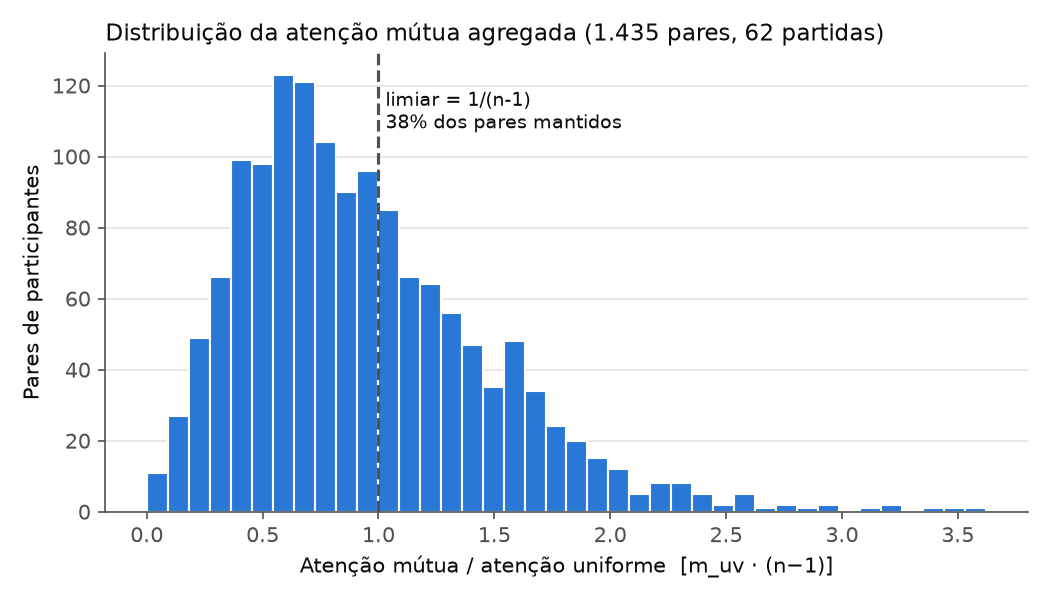
\includegraphics[width=\linewidth]{distribuicao_atencao.png}
\caption{Distribuição da atenção mútua normalizada pela atenção uniforme. A linha tracejada marca o
limiar adotado: 38\% dos 1.435 pares são mantidos.}
\label{fig:limiar}
\end{figure}

A Figura~\ref{fig:limiar} mostra a distribuição da atenção mútua com o limiar adotado. A distribuição
é unimodal e assimétrica à direita, e o limiar separa os pares com atenção acima do esperado sob
olhar uniforme.

%% ===================================================================
\section{Metodologia}

\textbf{Grafo desconexo.} Como o grafo tem 85 componentes e a maior possui 8 vértices, adotamos três
políticas:
\begin{itemize}
  \item medidas globais (graus, densidade, clusterização, triângulos) são calculadas sobre o grafo inteiro;
  \item diâmetro, raio e caminho médio são calculados por componente, em número de saltos, e agregados
  (máximo e média);
  \item a robustez é avaliada no grafo inteiro, já que 5\% de 8 vértices não é um número inteiro de
  vértices. O Apêndice~C do enunciado permite essa alternativa.
\end{itemize}

\textbf{Tempo de execução.} Cada medida é o tempo de parede de \texttt{time.perf\_counter}, com o
coletor de lixo desligado. Antes de medir, cada algoritmo é executado uma vez para aquecimento e para
calibrar o tamanho do lote: como no \texttt{timeit}, cada amostra executa o algoritmo $k$ vezes até
somar pelo menos 5\,ms e registra o tempo médio por execução. No grafo completo, usamos $n = 30$
amostras, e o intervalo de confiança de 95\% segue a Normal:
$\bar{x} \pm z_{0,975}\, s/\sqrt{n}$, com $z_{0,975} = 1{,}96$.
No estudo de escalabilidade, usamos subgrafos com as primeiras $8, 16, \ldots, 62$ partidas e
$n = 10$ amostras por ponto. Nesse caso, com $\sigma$ desconhecido, o intervalo segue a t-Student:
$\bar{x} \pm t_{0,975;\,9}\, s/\sqrt{n}$, com $t_{0,975;\,9} = 2{,}262$.
As medições foram feitas em um notebook com 2 núcleos e outros processos em execução, o que explica
alguns pontos atípicos.

\textbf{Reprodutibilidade.} Todos os sorteios usam a semente 224215945 (a matrícula).

%% ===================================================================
\section{Resultados -- Parte I}

A Tabela~\ref{tab:parte1} reúne as medidas obrigatórias. Todas foram calculadas; a coluna
``Calc.'' atende à exigência de indicar o que foi ou não computado.

\begin{table}[t]
\caption{Medidas estruturais do G16 tratado.}
\label{tab:parte1}
\small
\begin{tabular}{p{4.6cm}rc}
\toprule
Medida & Valor & Calc. \\
\midrule
Vértices / arestas & 451 / 548 & sim \\
Grau mínimo / máximo / médio & 0 / 7 / 2,43 & sim \\
Distribuição de graus & Fig.~\ref{fig:graus} & sim \\
Densidade (grafo inteiro) & 0,0054 & sim \\
Densidade média por componente & 0,46 & sim \\
Componentes conexas & 85 & sim \\
\quad não triviais / vértices isolados & 64 / 21 & sim \\
Tamanho das componentes & Fig.~\ref{fig:graus} & sim \\
Diâmetro (máximo / média por comp.) & 5 / 2,67 & sim \\
Raio (grafo inteiro) & $\infty$ (desconexo) & sim \\
\quad raio por componente (mín.--máx. / média) & 1--3 / 1,70 & sim \\
Caminho médio (pares conectados) & 1,68 & sim \\
Clusterização média (todos / grau $\ge 2$) & 0,39 / 0,55 & sim \\
Transitividade global & 0,38 & sim \\
Triângulos & 161 & sim \\
Visualização & Fig.~\ref{fig:grafo} & sim \\
\bottomrule
\end{tabular}
\end{table}

\begin{figure}[t]
\centering
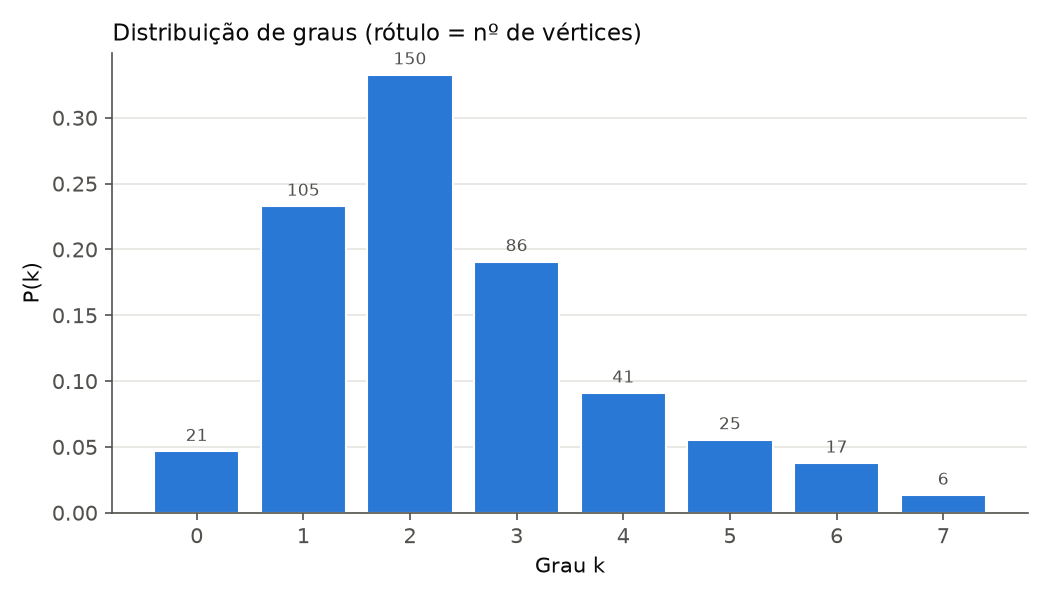
\includegraphics[width=0.49\linewidth]{parte1_distribuicao_graus.png}
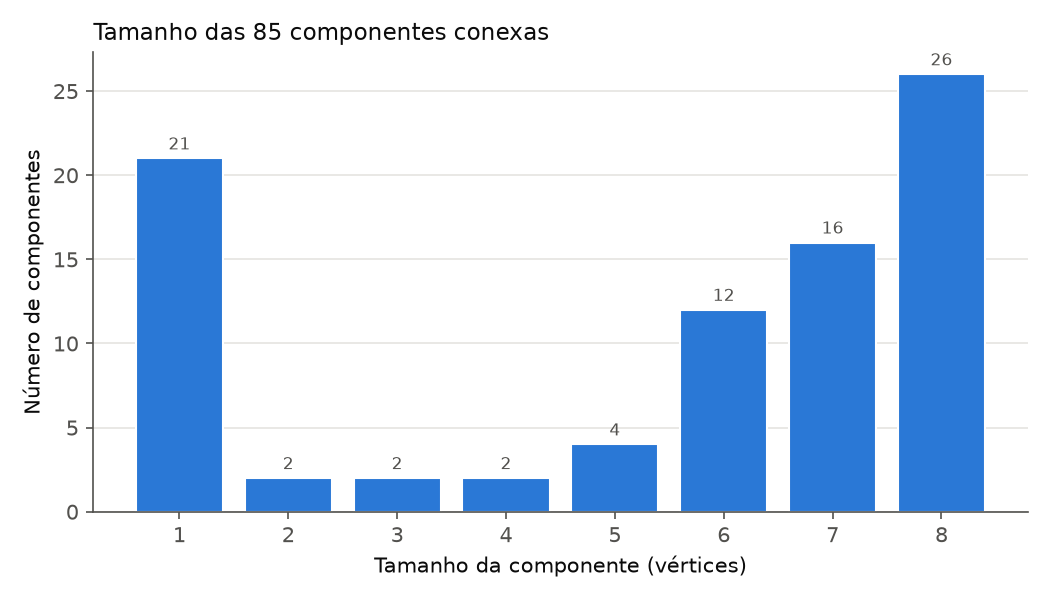
\includegraphics[width=0.49\linewidth]{parte1_tamanho_componentes.png}
\caption{Esquerda: distribuição de graus, unimodal com pico em $k=2$. Direita: tamanho das 85
componentes; 26 delas têm 8 vértices, o máximo possível.}
\label{fig:graus}
\end{figure}

\begin{figure*}[t]
\centering
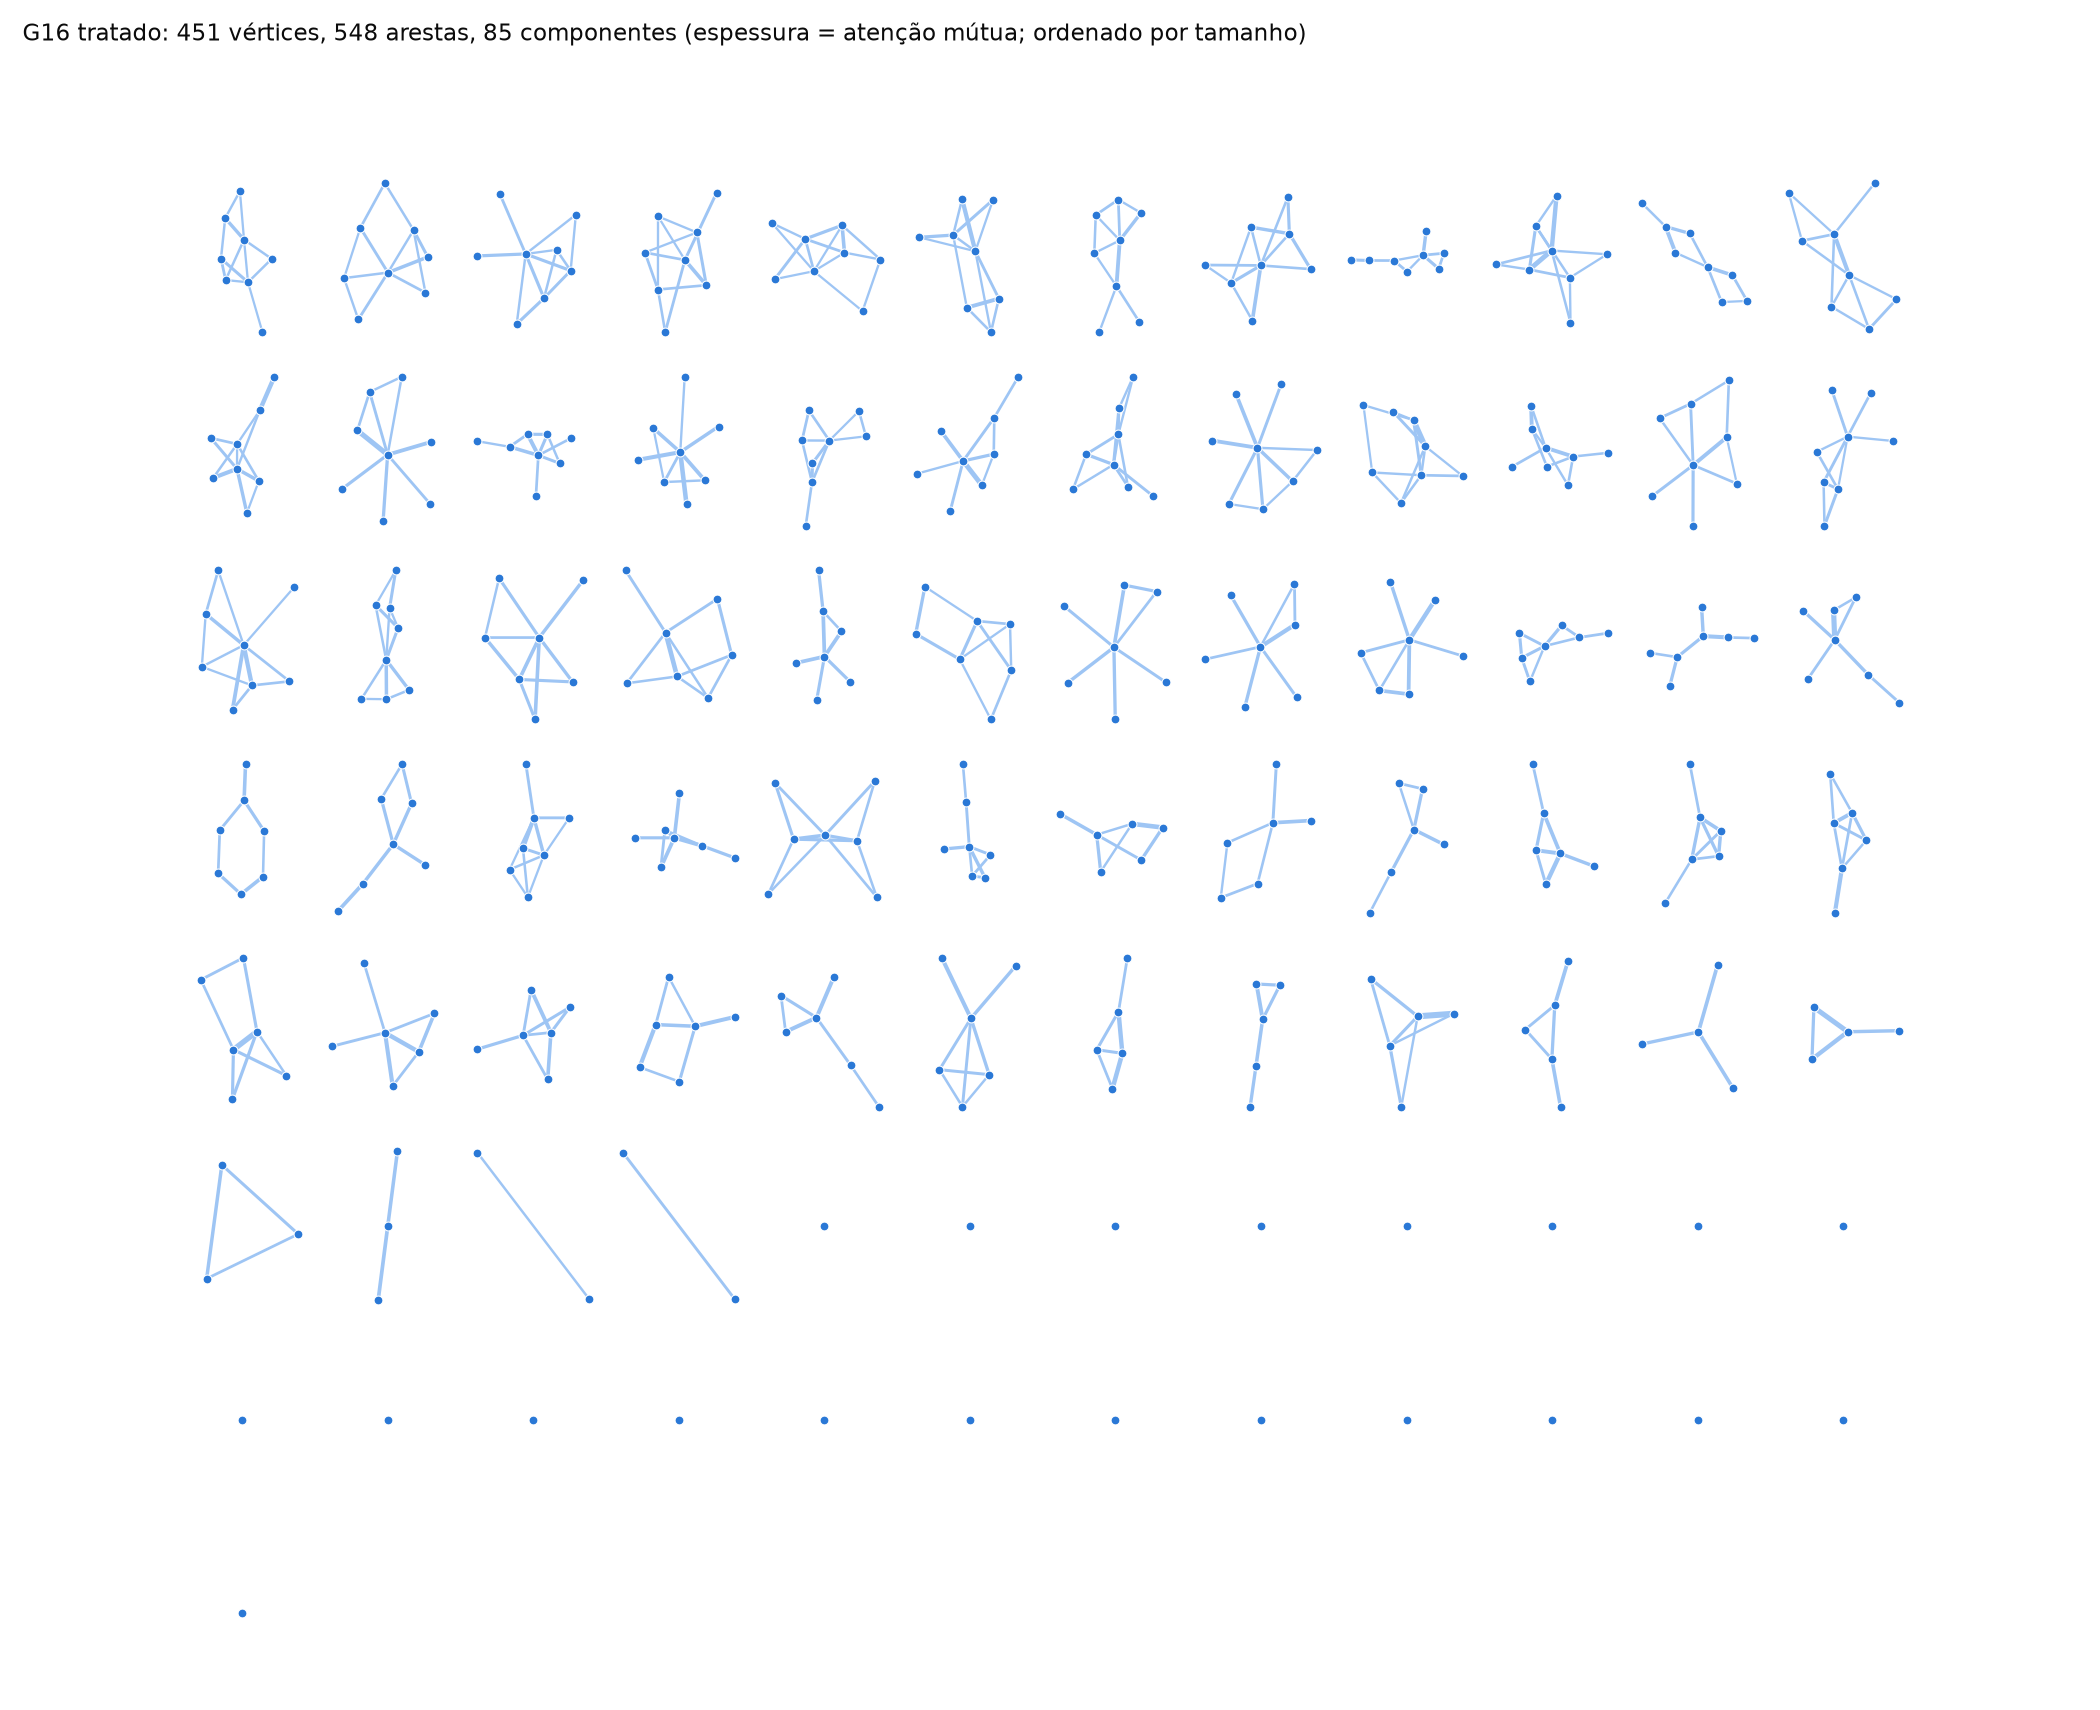
\includegraphics[width=0.85\textwidth]{parte1_grafo.png}
\caption{O grafo inteiro, com cada componente desenhada separadamente e em ordem de tamanho.
A espessura da aresta é proporcional à atenção mútua. Várias componentes têm forma de estrela em
torno de um vértice de grau alto.}
\label{fig:grafo}
\end{figure*}

\textbf{Comentários.}
\begin{itemize}
  \item A densidade global de 0,0054 é baixa apenas porque as partidas não se conectam entre si.
  Dentro de cada componente, a densidade média é 0,46.
  \item Há 64 componentes não triviais para 62 partidas: em duas partidas, o limiar separou subgrupos
  que quase não se olham.
  \item Distâncias pequenas (diâmetro máximo 5, caminho médio 1,68) e clusterização alta
  (0,39) são esperadas em grupos de até 8 pessoas.
  \item Os 6 vértices de grau 7 estão ligados a todos os demais jogadores de partidas de 8 pessoas.
  Eles aparecem como centros de estrela na Figura~\ref{fig:grafo} e motivam a
  Seção~\ref{sec:descoberta}.
\end{itemize}

%% ===================================================================
\section{Resultados -- Parte II}

Todos os algoritmos foram implementados do zero (\texttt{src/algoritmos.py}). As árvores geradoras e
os caminhos mínimos usam o peso $d_{uv}$. Cada implementação foi conferida com o NetworkX, e os 13
testes de validação passaram. A Tabela~\ref{tab:alg} resume o resultado de cada algoritmo no G16.

\begin{table*}[t]
\caption{Algoritmos da disciplina: complexidade teórica, resultado no G16 e tempo observado
(média, desvio padrão e IC 95\% pela Normal, $n=30$).}
\label{tab:alg}
\small
\begin{tabular}{llp{6.6cm}rrr}
\toprule
Algoritmo & Teórica & Resultado no G16 & Média (ms) & DP (ms) & IC 95\% (ms) \\
\midrule
BFS (todas as comp.) & $O(V+E)$ & 85 árvores; da origem R61\_P5 alcança 8 vértices, profundidade 1 & 0,240 & 0,038 & [0,226; 0,253] \\
DFS (iterativa) & $O(V+E)$ & 85 árvores de busca & 0,240 & 0,020 & [0,232; 0,247] \\
Eulerianidade & $O(V+E)$ & não euleriano (222 vértices de grau ímpar; desconexo); por comp.: 5 eulerianas, 21 semi, 38 não & 0,060 & 0,006 & [0,057; 0,062] \\
Dijkstra (heap) & $O((V+E)\log V)$ & aplicável (pesos $\ge 0$); da origem, 8 vértices alcançados & 0,0066 & 0,0027 & [0,0057; 0,0076] \\
Bellman-Ford & $O(V \cdot E)$ & aplicável, mas desnecessário; mesmas distâncias, sem ciclo negativo & 26,71 & 0,70 & [26,46; 26,97] \\
Floyd-Warshall & $O(V^3)$ & $451 \times 451$; 1.304 pares conectados, distância média 1,28 & 433,3 & 134,4 & [385,2; 481,4] \\
Tarjan (CFC, dirigido) & $O(V+E)$ & 165 componentes fortemente conexas (101 unitárias) & 0,586 & 0,042 & [0,571; 0,601] \\
Tarjan (articulações/pontes) & $O(V+E)$ & 72 pontos de articulação, 112 pontes & 0,493 & 0,036 & [0,480; 0,506] \\
Kruskal (união-busca) & $O(E\log E)$ & floresta com $366 = 451 - 85$ arestas, peso 272,17 & 0,418 & 0,031 & [0,407; 0,429] \\
Prim (heap) & $O(E\log V)$ & mesma floresta (mesmo peso) & 0,312 & 0,028 & [0,301; 0,322] \\
\bottomrule
\end{tabular}
\end{table*}

\textbf{Observações sobre aplicabilidade.}
\begin{itemize}
  \item Dijkstra e Bellman-Ford se aplicam porque os pesos são não negativos. Sem pesos negativos,
  porém, o Bellman-Ford não traz vantagem: dá as mesmas distâncias e custa cerca de 4.000 vezes mais.
  \item No Floyd-Warshall, o laço em $k$ é explícito e a atualização dos $V^2$ pares de cada rodada é
  vetorizada com NumPy. O custo continua $O(V^3)$.
  \item O algoritmo de Tarjan~\cite{tarjan1972depth} foi aplicado em duas versões: componentes
  fortemente conexas no grafo dirigido, e pontos de articulação e pontes no grafo não dirigido.
  \item Como o grafo é desconexo, Kruskal e Prim produzem uma \emph{floresta} geradora mínima.
  Minimizar $d = 1-m$ equivale a maximizar a atenção total.
\end{itemize}

\begin{figure}[t]
\centering
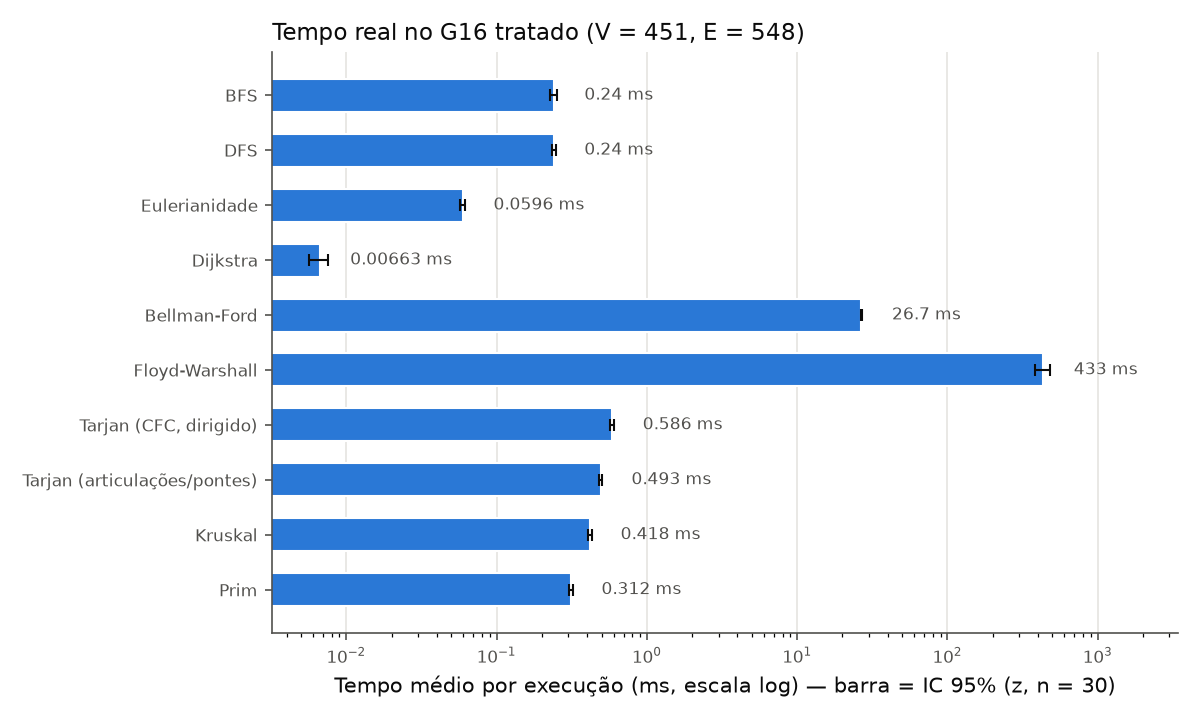
\includegraphics[width=\linewidth]{parte2_tempos.png}
\caption{Tempo médio por execução no grafo completo (escala logarítmica), com IC 95\% ($z$, $n=30$).}
\label{fig:tempos}
\end{figure}

\begin{figure*}[t]
\centering
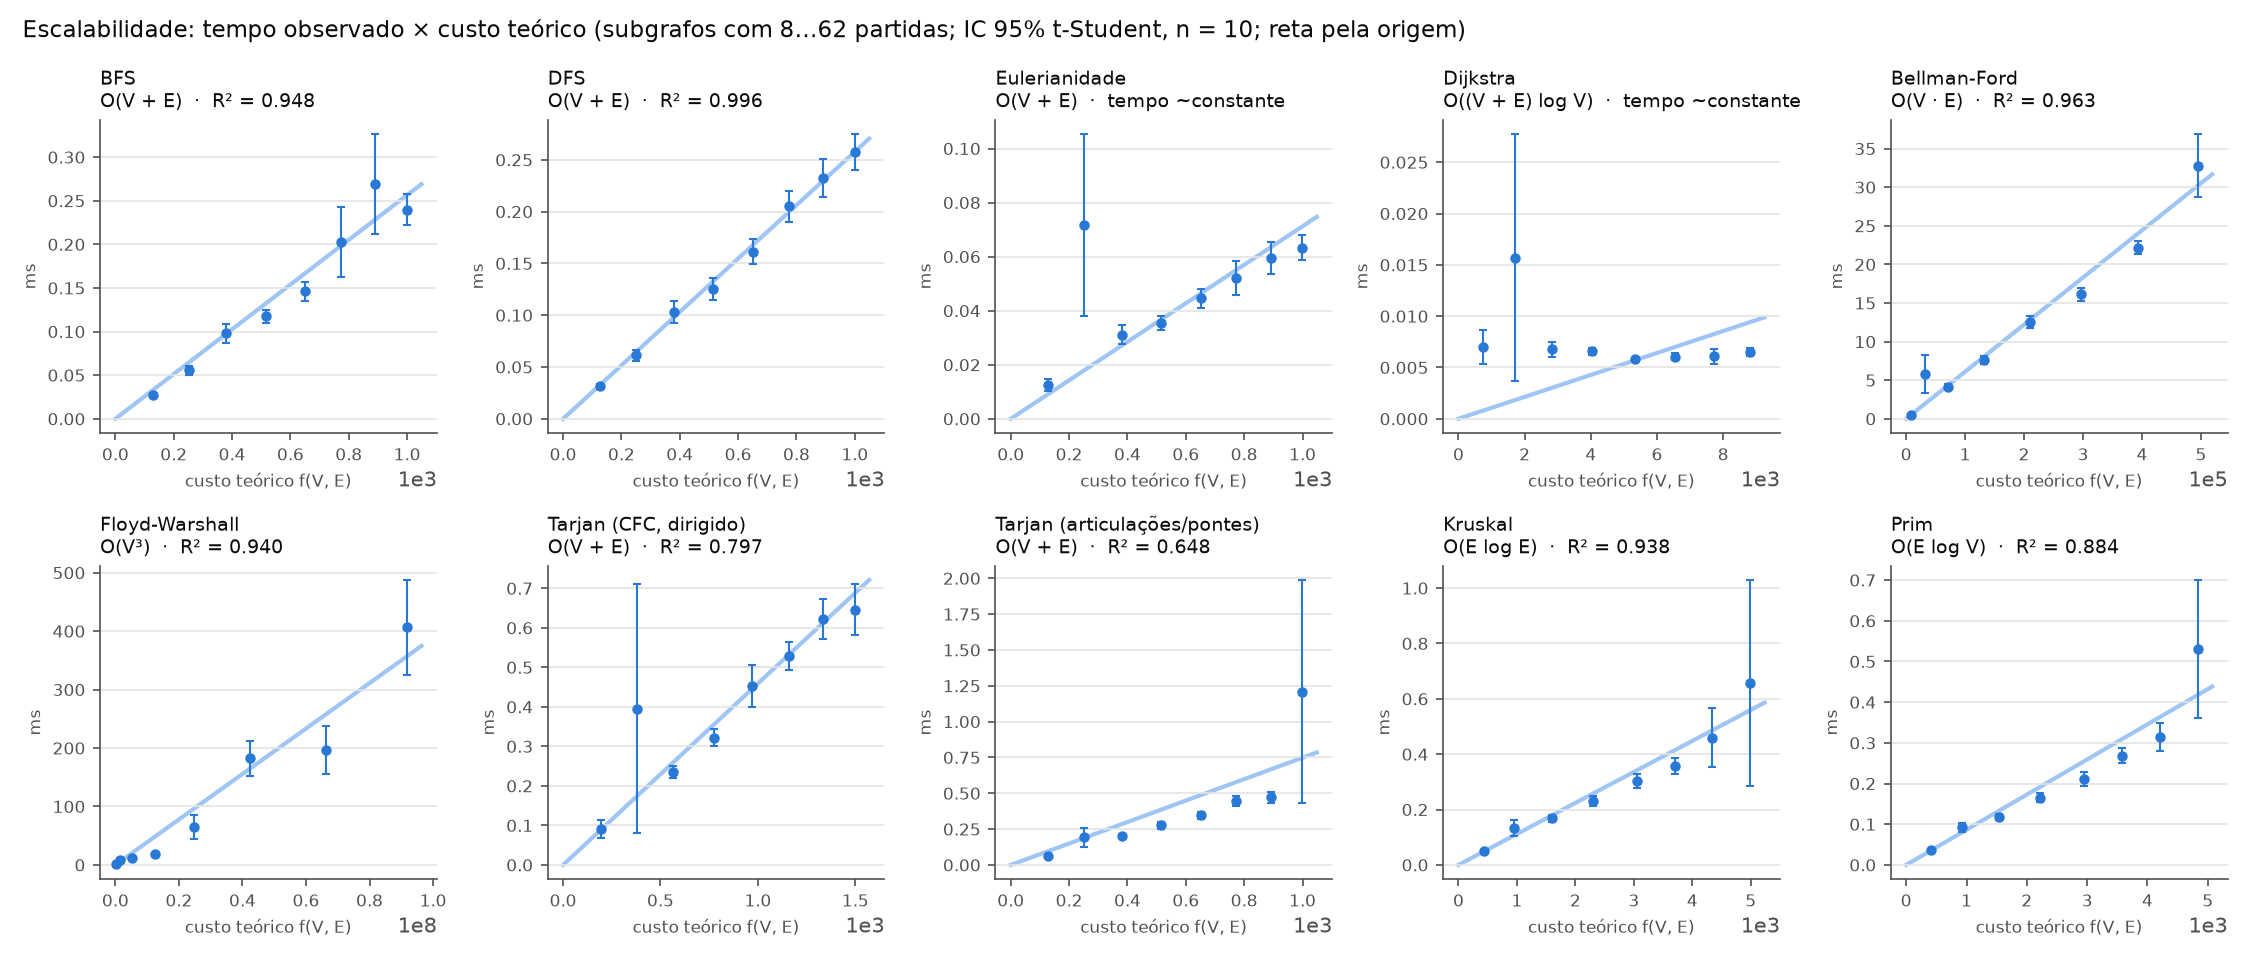
\includegraphics[width=\textwidth]{parte2_escalabilidade.png}
\caption{Escalabilidade: tempo observado contra a função de custo teórica, em subgrafos com 8 a 62
partidas (IC 95\% pela t-Student, $n=10$), com reta ajustada pela origem.}
\label{fig:escala}
\end{figure*}

\textbf{Teórico $\times$ observado.} A Figura~\ref{fig:tempos} confirma a ordem esperada de custos:
os algoritmos lineares levam menos de 1\,ms; o Bellman-Ford, cerca de 27\,ms; e o Floyd-Warshall,
cerca de 0,4\,s. Na Figura~\ref{fig:escala}, o tempo cresce linearmente com a função de custo
teórica em BFS ($R^2 = 0{,}95$), DFS (0,996), Bellman-Ford (0,96), Floyd-Warshall (0,94),
Kruskal (0,94) e Prim (0,88). Os $R^2$ menores de Eulerianidade, das duas versões de Tarjan e de
alguns pontos de Prim vêm de pontos isolados com intervalo de confiança largo, típicos de
interferência de outros processos; os demais pontos acompanham a reta.

O caso mais interessante é o \textbf{Dijkstra}, cujo tempo é praticamente constante (cerca de
6\,$\mu$s), qualquer que seja o tamanho do grafo. A busca termina quando esgota a componente da
origem, que tem no máximo 8 vértices. Logo, o custo real depende do tamanho da componente, e não de
$V$ e $E$ totais. O Bellman-Ford clássico, ao contrário, percorre todos os arcos $V-1$ vezes e cresce
conforme o previsto.

%% ===================================================================
\section{Resultados -- Parte III}

\subsection{Small-world}

\textbf{Método.} Comparamos o grafo com grafos aleatórios equivalentes~\cite{watts1998collective},
resumindo a comparação pelo índice
$\sigma = (C/C_{\text{rand}})/(L/L_{\text{rand}})$~\cite{humphries2008network}, em que valores de
$\sigma > 1$ indicam small-world. A clusterização, o caminho médio (BFS) e o gerador $G(n,m)$ de
Erdős--Rényi~\cite{erdos1959random} foram implementados por nós, e a clusterização e o caminho médio
conferem com o NetworkX. Cada componente com $n \ge 4$ que não é completa (60 das 64) foi comparada
com 200 grafos ER conexos de mesmos $n$ e $m$, obtidos por amostragem com rejeição.

\begin{figure*}[t]
\centering
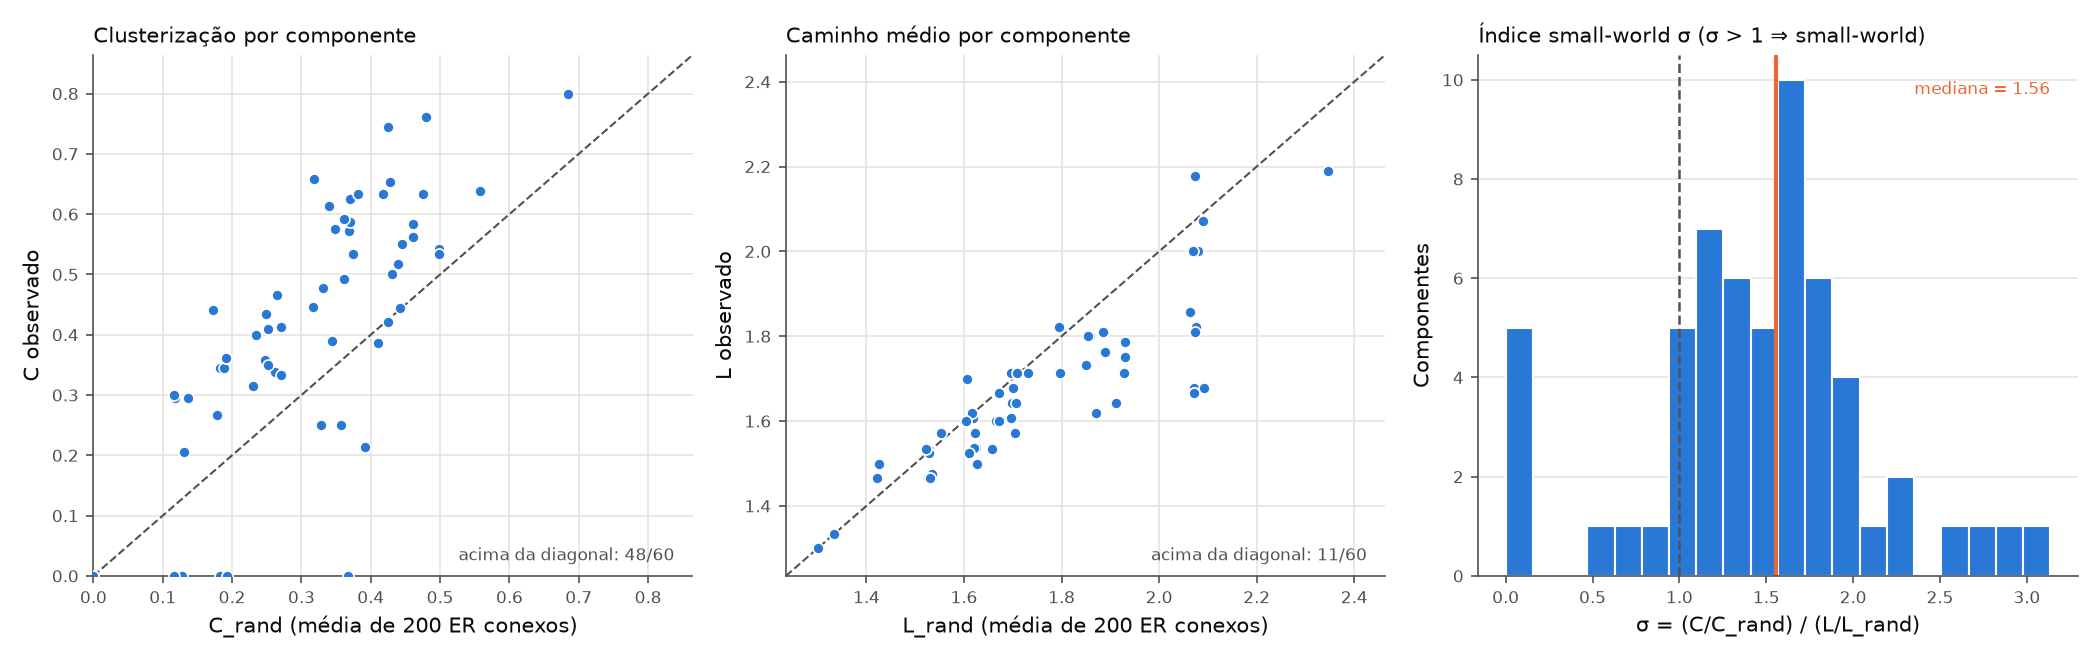
\includegraphics[width=\textwidth]{parte3_small_world.png}
\caption{Small-world por componente: $C$ contra $C_{\text{rand}}$, $L$ contra $L_{\text{rand}}$
(diagonal = igual ao aleatório) e histograma de $\sigma$.}
\label{fig:sw}
\end{figure*}

\textbf{Resultado} (Figura~\ref{fig:sw}). Na média das componentes:
\begin{itemize}
  \item $C = 0{,}414$ contra $C_{\text{rand}} = 0{,}313$, ou seja, $C/C_{\text{rand}} = 1{,}32$;
  \item $L = 1{,}669$ contra $L_{\text{rand}} = 1{,}762$, ou seja, $L/L_{\text{rand}} = 0{,}95$;
  \item $\sigma$ agregado de 1,40 e mediana de 1,56; $\sigma > 1$ em 49 de 58 componentes;
  \item $C$ só é significativamente maior que o aleatório (teste empírico, $p<0{,}05$) em
  9 de 60 componentes.
\end{itemize}

\textbf{Resposta.} Há \emph{indícios fracos}: o caminho médio é igual ou menor que o aleatório, mas a
clusterização não é ``muito maior'', como exige a definição. Faz sentido para este grafo: em grupos
de 5 a 8 pessoas, qualquer grafo razoavelmente denso já tem caminhos curtos (densidade média 0,43) e
clusterização alta mesmo ao acaso. Na prática, se a rede fosse small-world, a informação percorreria
a partida em poucos passos ao mesmo tempo em que se formariam subgrupos coesos. Aqui, o primeiro
efeito decorre do tamanho do grupo, e o segundo é modesto.

\textbf{Alerta.} A comparação \emph{global} do grafo inteiro com um ER $G(451, 548)$ resulta em
$\sigma = 356$, pois $C_{\text{rand}} = 0{,}004$ e $L_{\text{rand}} = 6{,}5$. Esse valor é um
artefato: o ER forma uma componente gigante que o G16 não tem. Por isso, adotamos a comparação por
componente.

\subsection{Lei de potência}

\textbf{Método.} Seguimos o procedimento de Clauset et al.~\cite{clauset2009power}:
\begin{itemize}
  \item histograma e distribuição complementar acumulada (CCDF) em escala log-log, com regressão linear;
  \item ajuste de $p(k) \propto k^{-\alpha}$ por máxima verossimilhança discreta, com $k_{\min}$
  escolhido pela menor distância de Kolmogorov--Smirnov (KS);
  \item $p$-valor de aderência por bootstrap semiparamétrico com 1.000 reamostragens;
  \item testes de razão de verossimilhança de Vuong~\cite{vuong1989likelihood} contra a
  exponencial e contra a Poisson truncadas.
\end{itemize}

\begin{figure}[t]
\centering
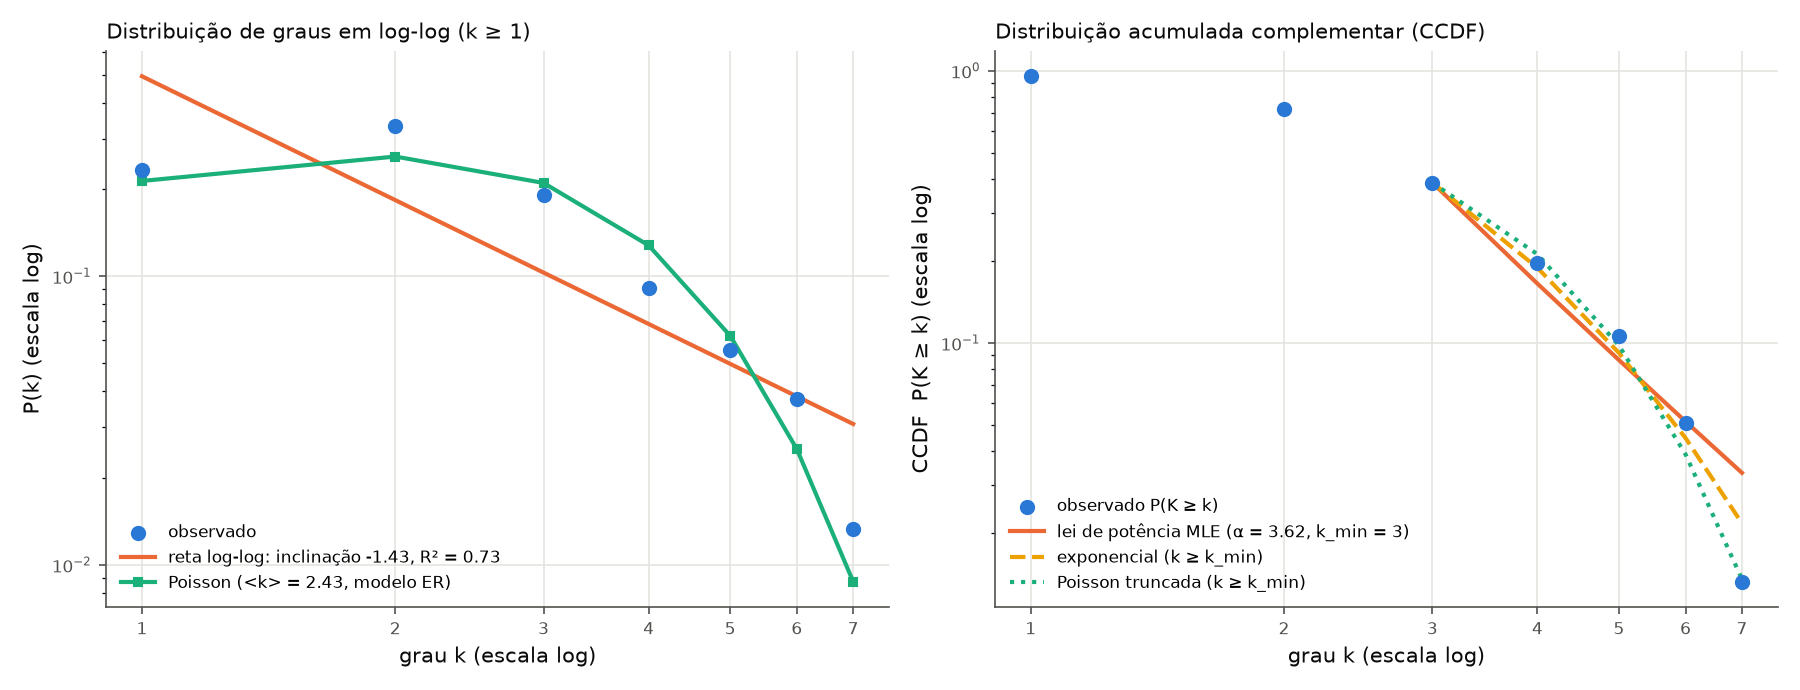
\includegraphics[width=\linewidth]{parte3_lei_potencia.png}
\caption{Distribuição de graus em escala log-log (esquerda) e CCDF com os modelos ajustados
para $k \ge k_{\min}$ (direita).}
\label{fig:pl}
\end{figure}

\textbf{Resultado} (Figura~\ref{fig:pl}).
\begin{itemize}
  \item Os graus variam de 1 a 7 entre os vértices não isolados: menos de uma década, o que já
  impede uma cauda pesada.
  \item A razão entre variância e média é 0,92, assinatura da Poisson típica de grafos ER.
  \item Em log-log, $P(k)$ não é linear ($R^2 = 0{,}73$) e cresce até $k=2$. Na CCDF, a forma
  exponencial ajusta melhor ($R^2 = 0{,}97$) que a lei de potência ($R^2 = 0{,}82$).
  \item O ajuste de máxima verossimilhança dá $\alpha = 3{,}62 \pm 0{,}20$ para $k \ge 3$, com
  KS $= 0{,}083$, mas o bootstrap rejeita a hipótese ($p = 0{,}00$).
  \item A lei de potência perde para a exponencial ($R = -10{,}8$; $p < 0{,}001$) e para a Poisson
  ($R = -13{,}1$; $p = 0{,}002$).
\end{itemize}

\textbf{Resposta.} \emph{Não} há lei de potência, e o resultado é coerente com o tratamento: o grau de
cada vértice é limitado pelo tamanho da partida ($k \le n-1 \le 7$), o que impede hubs globais.

\subsection{Robustez}

\textbf{Método.} Removemos $r = \lceil 0{,}05 \times 451 \rceil = 23$ vértices do grafo inteiro e
medimos:
\begin{itemize}
  \item (A) o tamanho da maior componente, absoluto e relativo ao original ($S/S_0$);
  \item (B) o número de componentes;
  \item (C) o caminho médio e a eficiência global $E = \frac{1}{N(N-1)}\sum 1/d_{uv}$~\cite{latora2001efficient};
  \item (D) a fração de vértices isolados;
  \item (E*) a fração de pares conectados preservada. Acrescentamos essa métrica porque a A não
  distingue cenários neste grafo.
\end{itemize}
Na remoção aleatória, fizemos 50 repetições. No ataque, usamos um ranking fixo calculado no grafo
original, por grau e por betweenness. Os dois rankings compartilham 15 dos 23 vértices.

\begin{table}[t]
\caption{Robustez à remoção de 5\% dos vértices ($r=23$). Aleatória: média $\pm$ desvio padrão
(50 repetições).}
\label{tab:rob}
\small
\begin{tabular}{lrrrr}
\toprule
Métrica & Orig. & Aleatória & Grau & Betw. \\
\midrule
A: maior comp. ($S/S_0$) & 1,00 & 1,00 $\pm$ 0 & 1,00 & 1,00 \\
B: componentes & 85 & 89,7 $\pm$ 2,7 & 124 & 138 \\
C: caminho médio & 1,685 & 1,678 $\pm$ 0,011 & 1,778 & 1,647 \\
C: eficiência ($\times 10^{3}$) & 8,91 & 8,77 $\pm$ 0,11 & 7,11 & 6,90 \\
D: fração de isolados & 0,047 & 0,059 $\pm$ 0,007 & 0,136 & 0,157 \\
E*: pares conectados & 1,000 & 0,881 $\pm$ 0,011 & 0,732 & 0,673 \\
\bottomrule
\end{tabular}
\end{table}

\begin{figure*}[t]
\centering
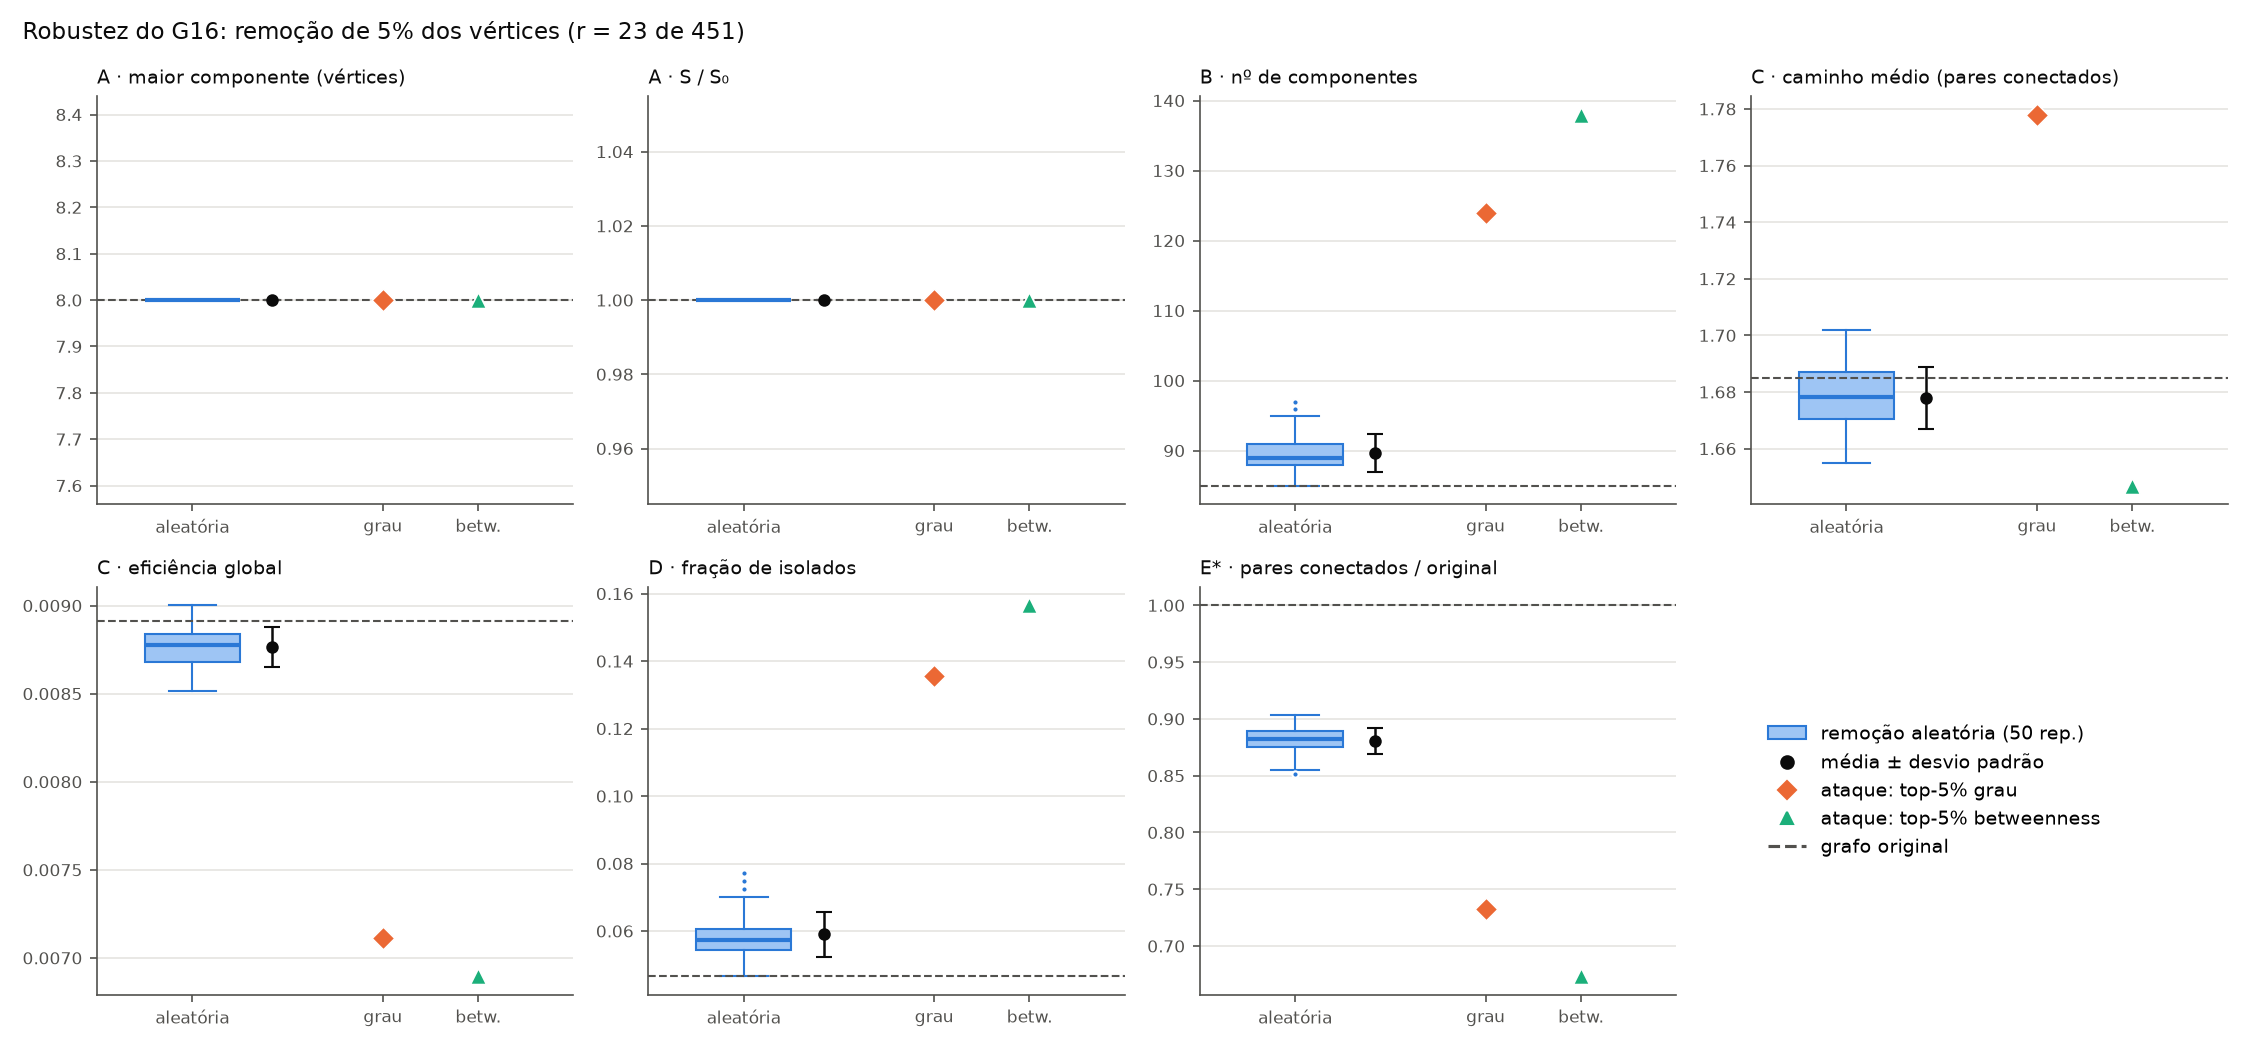
\includegraphics[width=0.85\textwidth]{parte3_robustez_boxplots.png}
\caption{Boxplots da remoção aleatória (50 repetições, com média $\pm$ desvio padrão) e valores dos
ataques por grau e por betweenness. A linha tracejada indica o grafo original.}
\label{fig:rob}
\end{figure*}

\begin{figure*}[t]
\centering
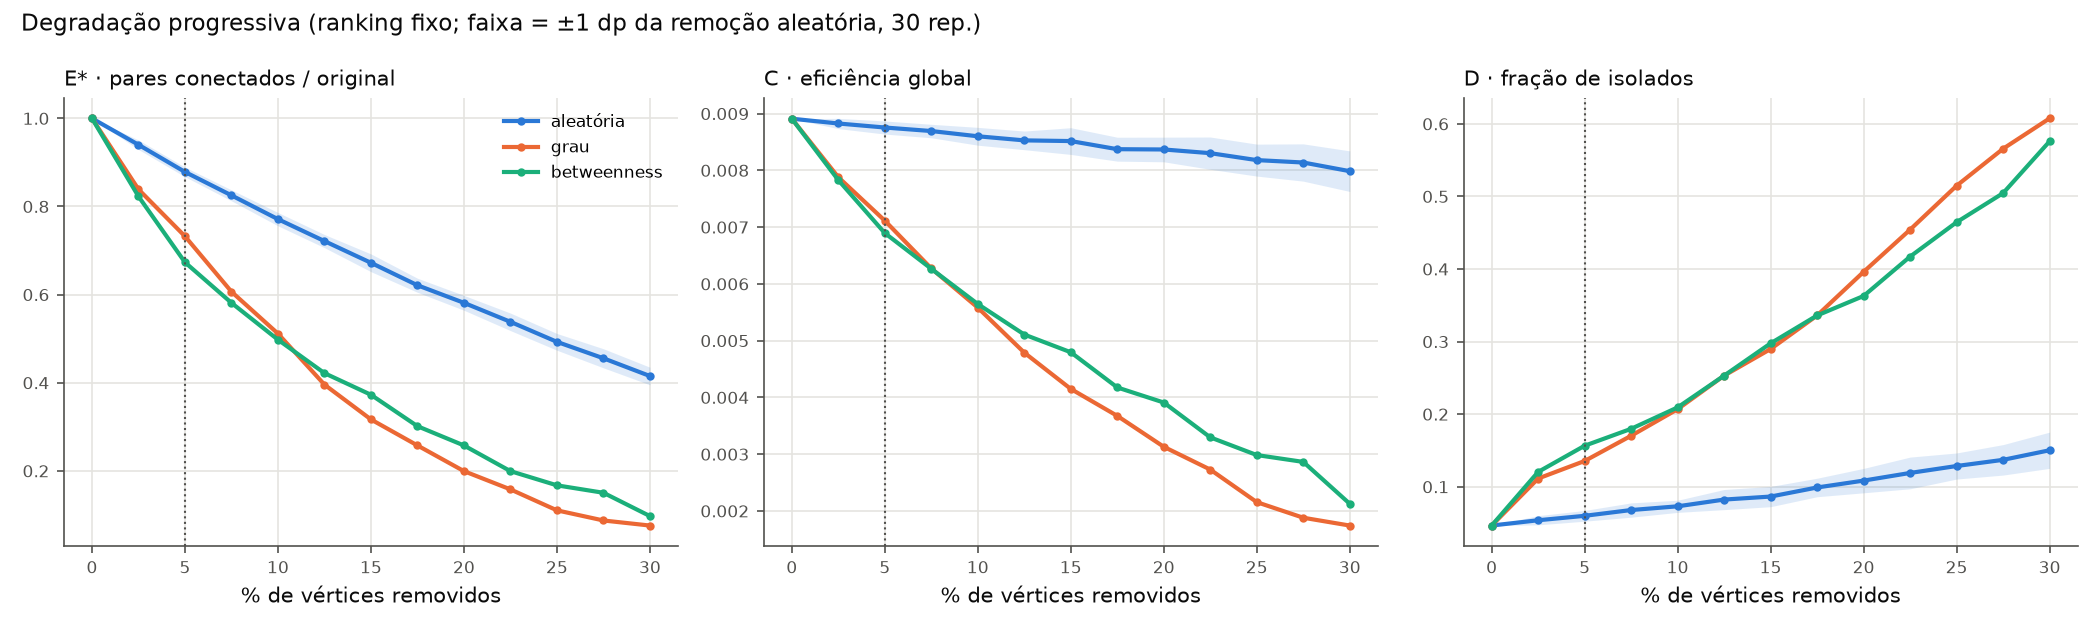
\includegraphics[width=\textwidth]{parte3_robustez_curvas.png}
\caption{Degradação progressiva com remoção de 0 a 30\% dos vértices. A faixa indica $\pm 1$ desvio
padrão da remoção aleatória (30 repetições).}
\label{fig:curvas}
\end{figure*}

\textbf{Resultado} (Tabela~\ref{tab:rob} e Figuras~\ref{fig:rob} e~\ref{fig:curvas}).
\begin{itemize}
  \item A métrica A não se altera em nenhum cenário: com 26 componentes de tamanho 8, remover 23
  vértices nunca atinge todas.
  \item Na \textbf{remoção aleatória}, o grafo mantém 88\% dos pares conectados. Só a perda dos
  pares que têm um extremo removido já explica cerca de $1 - 0{,}95^2 \approx 9{,}8\%$; a fragmentação
  adicional fica em torno de 2\%. O número de componentes sobe pouco (de 85 para 90) e os isolados
  vão de 4,7\% para 5,9\%.
  \item No \textbf{ataque}, os pares preservados caem para 73\% (grau) e 67\% (betweenness), os
  isolados quase triplicam e as componentes passam de 124 a 138. Esses valores ficam entre 11 e 18
  desvios padrão além da distribuição aleatória.
  \item O caminho médio sobe com o ataque por grau (removem-se centros de estrela, e os caminhos
  passam a dar voltas) e cai com o ataque por betweenness (a rede se fragmenta e restam só pares
  próximos). Por isso, a eficiência é a métrica de distância mais informativa.
  \item As curvas mostram que a diferença se mantém em todas as frações removidas.
\end{itemize}

\textbf{Resposta.} O grafo é \emph{robusto à remoção aleatória} e \emph{vulnerável ao ataque
direcionado}: a perda de pares conectados sob ataque é de 2,3 a 2,7 vezes a da remoção aleatória. É o padrão descrito por Albert et
al.~\cite{albert2000error} para redes com vértices críticos. Aqui, porém, a vulnerabilidade é
\emph{local}: cada partida depende do seu próprio vértice central, como se verá na próxima seção.

\subsection{Descoberta mais interessante: o jogador focal}
\label{sec:descoberta}

Usando a versão dirigida e os dados temporais brutos, verificamos se a atenção de cada partida se
concentra em um jogador:
\begin{itemize}
  \item Em \textbf{32 das 62 partidas}, há um jogador que \emph{todos} os demais olham acima do
  uniforme; ele tem grau de entrada $n-1$ no grafo dirigido.
  \item Em média, o mais olhado recebe \textbf{2,0 vezes} a parcela uniforme ($27{,}8\%$ contra $13{,}9\%$).
  \item A atenção \emph{recebida} é desigual (Gini médio de 0,27), enquanto a \emph{emitida} é quase
  igual entre os jogadores (Gini de 0,03; teste de Wilcoxon, $p<0{,}001$). Todos olham para os colegas
  por um tempo parecido, mas para poucos deles.
  \item \textbf{O papel é persistente}: dividindo cada partida em três terços, o mais olhado é o mesmo
  nos três em \textbf{42 das 62 partidas}, contra 1,2 esperado ao acaso ($p \approx 10^{-4}$ em 10.000
  simulações). A correlação de Spearman entre o primeiro e o último terço tem mediana de 0,86
  (Figura~\ref{fig:focal}).
  \item A reciprocidade dos arcos (0,41) é apenas um pouco maior que o esperado ao acaso (0,36): a
  atenção é em grande parte assimétrica.
\end{itemize}

\begin{figure*}[t]
\centering
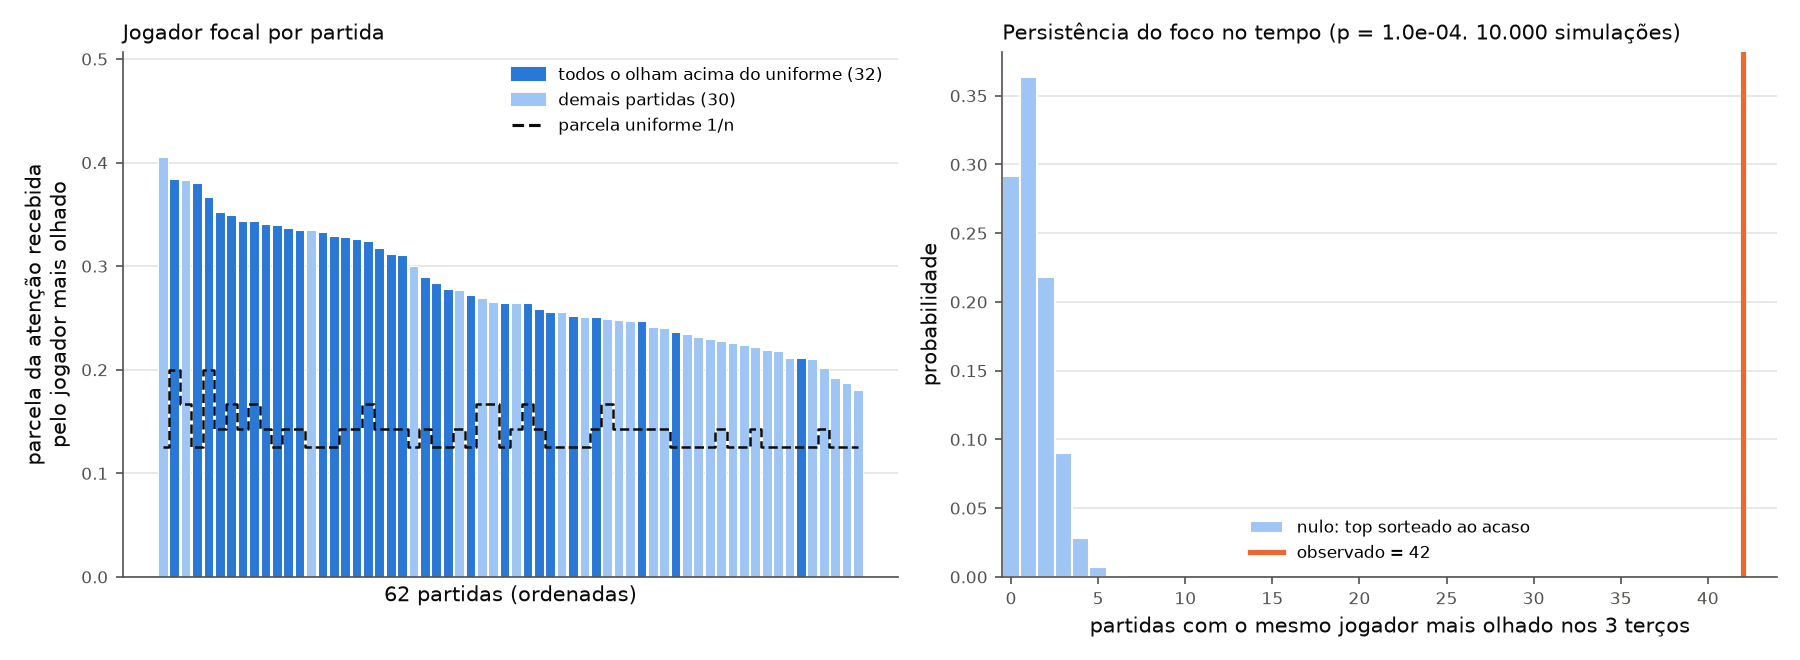
\includegraphics[width=0.85\textwidth]{parte3_descoberta.png}
\caption{Esquerda: parcela da atenção recebida pelo jogador mais olhado de cada partida; as barras
escuras marcam as partidas em que todos o olham acima do uniforme. Direita: número de partidas com o
mesmo jogador mais olhado nos três terços, comparado com o acaso.}
\label{fig:focal}
\end{figure*}

O jogador focal explica os hubs e as estrelas da Parte~I, a eficácia do ataque por grau e a
semelhança com o modelo BA (próxima seção). Uma limitação é que a posição dos jogadores à mesa ou em
relação à câmera, que os dados não registram, pode contribuir para o efeito.

\subsection{Extra: aproximação a modelos clássicos}

\textbf{Método.} Para cada uma das 60 componentes com $n \ge 4$, geramos 200 grafos de cada modelo
com o mesmo tamanho:
\begin{itemize}
  \item ER: $G(n,m)$, com o mesmo número de arestas;
  \item BA~\cite{barabasi1999emergence}: $m_{BA}$ arestas por novo vértice, com
  $m_{BA}(n-m_{BA}) \approx m$;
  \item WS: anel com $k \approx 2m/n$ vizinhos e probabilidade de religação $p = 0{,}1$.
\end{itemize}
A distância de variação total (TV) mede a diferença entre as distribuições de graus agregadas;
0 indica distribuições idênticas.

\begin{table}[t]
\caption{Observado contra modelos clássicos (médias sobre as 60 componentes).}
\label{tab:modelos}
\small
\begin{tabular}{lrrrrr}
\toprule
 & $C$ & $L$ & DP grau & Centraliz. & TV graus \\
\midrule
Observado & 0,414 & 1,669 & 1,28 & 0,578 & -- \\
ER & 0,345 & 1,692 & 1,00 & 0,358 & 0,187 \\
\textbf{BA} & 0,325 & 1,739 & 1,13 & 0,502 & \textbf{0,037} \\
WS ($p{=}0{,}1$) & 0,192 & 1,841 & 0,36 & 0,146 & 0,343 \\
\bottomrule
\end{tabular}
\end{table}

\begin{figure*}[t]
\centering
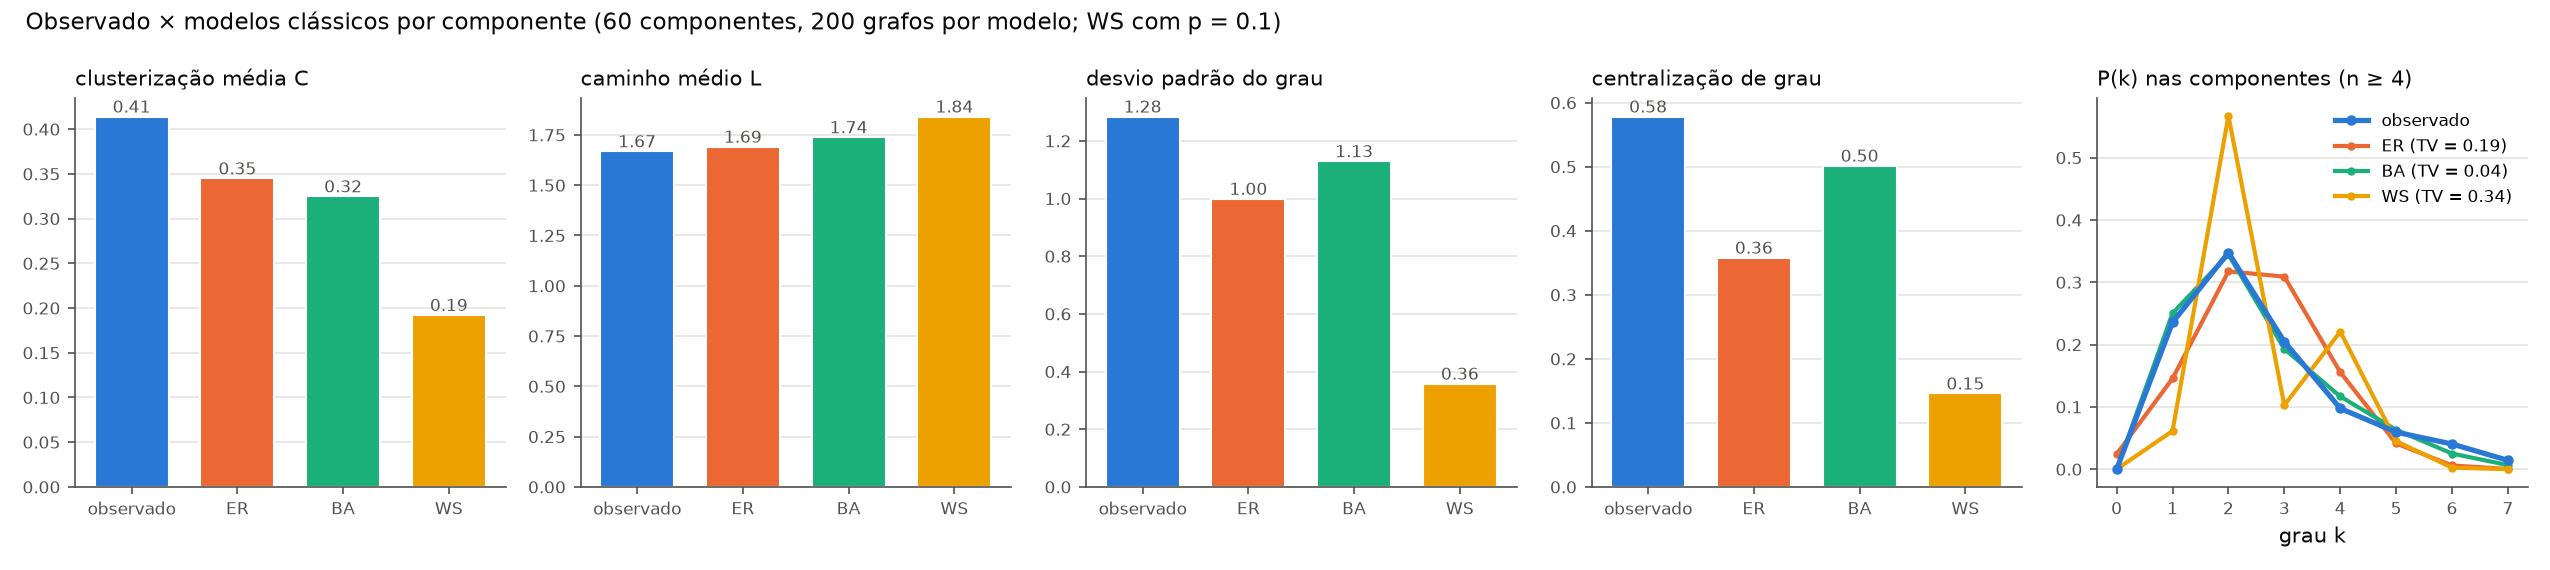
\includegraphics[width=\textwidth]{parte3_modelos.png}
\caption{Estatísticas médias por componente, observadas e de cada modelo, e distribuição de graus
agregada.}
\label{fig:modelos}
\end{figure*}

\textbf{Resultado} (Tabela~\ref{tab:modelos} e Figura~\ref{fig:modelos}).
\begin{itemize}
  \item O \textbf{BA é o modelo mais próximo}: tem a menor distância entre distribuições de graus
  (TV $= 0{,}04$) e a centralização de grau~\cite{freeman1978centrality} mais parecida
  (0,50 contra 0,58). Isso é coerente com o jogador focal, que se comporta como um hub de ligação
  preferencial.
  \item O ER subestima a heterogeneidade dos graus.
  \item O WS, com graus quase regulares, é o mais distante.
  \item Nenhum modelo reproduz a clusterização observada, que é maior que a de todos.
\end{itemize}
Concluímos que cada partida se aproxima de um BA pequeno com fechamento de triângulos adicional.
Globalmente, nenhum dos três modelos se aplica, porque nenhum gera 62 componentes disjuntas.

%% ===================================================================
\section{Discussão crítica}

\begin{itemize}
  \item \textbf{Efeito do tratamento.} Sem limiar, cada partida seria quase completa e as métricas
  seriam triviais. Com o limiar relativo $1/(n-1)$, o grafo reflete a atenção \emph{acima do esperado}.
  Ainda assim, a escolha é arbitrária, e a Tabela~\ref{tab:limiar} mostra que grau médio, número de
  isolados e componentes dependem dela. As conclusões qualitativas (componentes de no máximo 8
  vértices e ausência de lei de potência) valem para qualquer fator.
  \item \textbf{Grafo desconexo por construção.} Várias análises do enunciado pressupõem uma componente
  gigante: robustez na maior componente, small-world global e lei de potência. Aqui, elas exigiram
  adaptações (análise por componente, métrica E*) e cuidado com resultados enganosos, como o
  $\sigma = 356$ da comparação global.
  \item \textbf{Escala pequena.} Com 5 a 8 vértices por componente, testes estatísticos por componente
  têm pouco poder. Por isso, agregamos as 60 componentes e usamos modelos nulos simulados.
  \item \textbf{Tempos medidos.} Os tempos foram medidos em uma máquina compartilhada. As médias no
  grafo completo têm intervalos estreitos, mas a escalabilidade dos algoritmos mais rápidos tem pontos
  atípicos. O caso do Dijkstra mostra que a complexidade de pior caso pode superestimar muito o custo
  real em grafos desconexos.
  \item \textbf{Perda de informação temporal.} A agregação estática perde a dinâmica dentro de cada
  partida. A análise por terços recupera parte dela e mostra que o foco da atenção é estável.
\end{itemize}

%% ===================================================================
\section{Conclusão}

O G16, convertido em um grafo estático de atenção mútua, é formado por 85 componentes pequenas e
densas, uma ou duas por partida. As respostas às perguntas obrigatórias são:
\begin{enumerate}
  \item Há apenas indícios fracos de \emph{small-world}: os caminhos são tão curtos quanto ao acaso,
  mas a clusterização é só 1,3 vez a aleatória.
  \item A distribuição de graus \emph{não} segue lei de potência: é limitada e próxima da Poisson.
  \item A rede é robusta à remoção aleatória de 5\% dos vértices e vulnerável à remoção dos 5\% mais
  centrais, que preserva só 67--73\% dos pares conectados, contra 88\% na remoção aleatória.
  \item A descoberta mais interessante é o \emph{jogador focal}: um participante concentra a atenção
  do grupo, em geral de forma persistente ao longo da partida.
\end{enumerate}
No extra, o modelo Barabási--Albert é o que melhor descreve cada componente. Todos os algoritmos da
Parte~II foram implementados, validados e medidos; os tempos observados seguem as complexidades
teóricas, com a exceção explicada do Dijkstra.

\bibliographystyle{ACM-Reference-Format}
\bibliography{referencias}

\end{document}
